\section {生产计划与排程}
.
    \begin{center}
        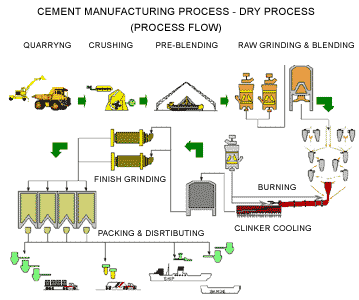
\includegraphics[scale=0.6]{process.png}
    \end{center}

    生产计划是关于企业生产运作系统总体方面的计划,是企业在计划期应达到的产品品种、质量、产量和产值等生产任务的计划和对产品生产进度的安排。它反映的并非某几个生产岗位或某一条生产线的生产活动,也并非产品生产的细节问题以及一些具体的机器设备、人力和其他生产资源的使用安排问题,而是指导企业计划期生产活动的纲领性方案。

\subsection {什么是生产计划}

    生产计划是指一方面为满足客户要求的三要素“交期、品质、成本”而计划;另一方面又使企业获得适当利益,而对生产的三要素“材料、人员、机器设备”的确切准备、分配及使用的计划。

    一个优化的生产计划必须具备以下三个特征:
        \begin{enumerate}
            \item  有利于充分利用销售机会,满足市场需求;
            \item  有利于充分利用盈利机会,实现生产成本最低化;
            \item  有利于充分利用生产资源,最大限度的减少生产资源的闲置和浪费。
        \end{enumerate}

    \subsubsection {生产计划的任务}

        \begin{enumerate}
            \item  要保证交货日期与生产量;
            \item  使企业维持同其生产能力相称的工作量(负荷)及适当开工率;
            \item  作为物料采购的基准依据;
            \item  将重要的产品或物料的库存量维持在适当水平;
            \item  对长期的增产计划,做人员与机械设备补充的安排。
        \end{enumerate}

    \subsubsection {生产计划的内容}

        \begin{enumerate}
            \item  生产什么东西—产品名称、零件名称;例:生产汽配行业的一种凸轮,名称代号:kj908
            \item  生产多少—数量或重量;因客人订单需要10000只,那实际生产应考虑到报废的产生,我们需要投产10500只,方能保证10000只的交货量。
            \item  在哪里生产—部门、单位;因生产制造行业的特性,显然我们主要是在生产部门完成指标,细化是在生产的各个工序班组间加工,包括:铸造、锻压、车床、铣床、高频淬火、磨床、清洗等。
            \item  要求什么时候完成—期间、交期。假如客人订单的交期要求在本月的20号,那么公司生产到完工应在20号之前完成,并且需要考虑物流运输的时间,以保证客户能在时限内收货。
        \end{enumerate}

    \subsubsection {生产计划的用途}

        \begin{enumerate}
            \item  物料需求计划的依据;
            \item  产能需求计划的依据;
            \item  其他相关计划的制定依据。
        \end{enumerate}

    \subsubsection {生产计划的种类}

        按不同性质划分,生产计划有各种类型见下表:

            \begin{itemize}
                \item  按时间周期分类
                    \begin{enumerate}
                        \item  2-3年长期计划,适用于产品群规划
                        \item  6-12月中期计划,适用于产品类别设计
                        \item  1-3月短期计划,是用于产品生产
                        \item  3-5周短期计划,适用于零件生产
                        \item  1-3日短期计划,适用于零件生产
                    \end{enumerate}

                \item  按计划层级/作用层级分类
                    \begin{enumerate}
                        \item  主生产计划(MPS)
                        \item  次生产计划(次MPS)
                    \end{enumerate}
            \end{itemize}

            此种分类常见与实际应用(尤其在有实体工厂的公司)。无论主、次生产计划(或主MPS、次MPS)其表现实体均是某个工序的计划安排。并选取其中最能体现公司经营运作和控制重点的工序作为其MPS(主MPS)的体现方式。一般制造业,均采用最后组装工序作为其MPS(主MPS)。

    \subsubsection {生产计划应满足的条件}
        \begin{enumerate}
            \item  计划应是综合考虑各有关因素的结果;
            \item  必须是有能力基础的生产计划;
            \item  计划的粗细必须符合活动的内容;
            \item  计划的下达必须在必要的时期。
        \end{enumerate}

\subsection {生产计划标准及层次}

    \subsubsection {生产计划的相关标准}

        \begin{enumerate}
            \item  作业计划的标准
                \begin{itemize}
                    \item  作业及加工的场所;例如:-------某某计划标准按照gb****** (当中的gb是指在中国境内生产的企业,*****是指行业名称);加工厂所可以是外协或本公司内生产,具体生产单位则是生产部。
                    \item  作业及加工的种类、顺序;例如:种类是指某种产品需要涉及到加工而产生的多少道工序,比喻上述所说凸轮加工,顺序则是指按完成凸轮制造而先做什么,后做什么,意思是将所有生产凸轮的工序进行排列。
                    \item  标准工时等。
                \end{itemize}

            \item  制程计划、余力计划的标准
                \begin{itemize}
                    \item  作业及加工制程别的负荷基准。
                    \item  作业及加工制程别的能力基准;制程计划是指制作与生产的工作程序,余力计划是指企业自身的生产能力与现有的生产能力差,比喻:本身企业每天生产1000只,那么现在我在生产800只,那么说明企业所提供的资源最大可以再生产200只,当超过总产量1000只,说明企业的生产能力饱和,这时如在增加生产那么我们必须相应增加设备与人力及各方面资源了。
                \end{itemize}

             \item  材料、零件计划的标准
                \begin{itemize}
                    \item  零件构成表及零件表;
                    \item  安排分区、供给分区;
                    \item  批量大小、产出率。
                \end{itemize}
            \item  日程计划的标准
                \begin{itemize}
                    \item  加工及装配基准日程表;
                    \item  批量。
                \end{itemize}
            \item  拟定库存计划的标准
                \begin{itemize}
                    \item  库存管理分区;
                    \item  订购周期;
                    \item  订购点、订购量;
                    \item  安全库存、最高库存、最低库存。
                \end{itemize}
        \end{enumerate}

        等等,上述计划标准,每逢变化时,应及时修正并予维持。

\subsection {生产计划指标}

    制定生产计划指标是生产计划的重要内容。为了有效的和全面的指导企业生产计划期的生产活动,生产计划应建立包括产品品种、产品质量、产品产量和产品产值的四类指标为主要内容的生产指标体系。

    1、产品品种指标

        产品品种指标是指企业在报告期内规定生产产品的名称、型号、规格和种类。它不仅反映企业对社会需求的满足能力,还反映了企业的专业化水平和管理水平。

        产品品种指标的确定首先要考虑市场需求和企业实力,按产品品种系列平衡法来确定。

    2、产品质量指标

        产品质量指标是衡量企业经济状况和技术发展水平的重要指标之一。产品质量受若干个质量控制参数控制。对质量参数的统一规定形成了质量技术标准,包括国际标准、国家标准、部颁标准、企业标准、企业内部标准等。

    3、产品产量指标

        产品产量指标是指企业在一定时期内生产的,并符合产品质量要求的实物数量。以实物量计算的产品产量,反映企业生产的发展水平,是制定和检查产量完成情况,分析各种产品质检比例关系和进行产品平衡分配,计算实物量生产指数的依据。

        确定产品产品指标主要采用盈亏平衡法、线性规划法等。

    4、产品产值指标

        产品产值指标是用货币表示的产量指标,能综合反映企业生产经营活动成果,以便进行不同行业间比较。根据具体内容和作用不同分为工业总产值、工业商品产值和工业增加值三种形式。

    生产计划的规划可以逐步精化为:

    \begin{enumerate}
        \item  无限能力计划。

      无限能力计划,指的就是在考虑出产计划、采购计划的时候,不考虑企业实际的出产能力,只管物料需求。这是大部门企业现在所采用的计划方法。这个方法的长处,就是操纵简便、轻易上手。但是,缺点也是很显著的。

        \begin{enumerate}
            \item  会增加企业的存货本钱。由于没有考虑到企业的实际出产能力,所以采购进来的良多材料,可能需要在企业中存一段时间才能用得着。要知道,这存放在企业里都是钱。放在企业中不仅会据有企业的资金,而且,对于企业的库存压力也不小,企业还要承担风险。如销售订单或者出产计划变更导致材料变为凝滞料的风险。
            \item  无法确定产品能否如期交货。由于没有考虑到企业的实际出产能力,所以,这个所谓的出产计划就会不断的进行变更。当一张出产订单由于产能的限制无法按时完成时,那其它的出产订单也不得不往后挪。所以,从无限能力计划上看不生产品能否及时交货。由于因为订单延期的不确定性,所以,最后,出产部分不得不像消防员一样,到处的去救火。
            \item  无限能力计划,不但会增加企业的存货本钱,而且会增加由于出产计划变更而造成的意外损失。企业若调整出产计划,则意味着还要调整职员铺排,有时候,可能因为产品的特殊性,还要调整出产线,那对企业的损失就大。
        \end{enumerate}

        \item  顺推法。

            顺推法指的是出产计划按照出产订单的前后逐一进行排。顺推法它考虑了企业的实际产能,所以,可以非常有效的解决由于无穷产能造成的题目。如企业可以根据出产计划来铺排采购计划及到料计划,从而减少企业库存的压力;由于考虑了实际产能,所以,基本上不会由于产能的题目而调整出产计划;同时,产品的交货期也有了一定的保障。但是,这个计划仍旧不是完美的,会出缺陷。
            \begin{enumerate}
                \item  若碰到紧急插单,就会无所适从。在企业中,根据客户重要性不同、产品的利润不同或者交货期的不同,紧急插单是常有的事情,特别是接单出产为主的企业。而顺推法的话,对于插单的敏感度不高。也就是说,利用顺推法把出产计划排好后,若碰到紧急订单的话,再重新排出产计划,那工作量会很大。一般企业的做法是,可能进行突击加班等手段,来解决这紧急订单的题目。
                \item  顺推法的工作量比较大。由于顺推法测算出产计划时,往往不能一次成功。有时候要在不同客户之间进行均衡、要最大程度的知足客户的交货需求,就需要不停的调整。而每调整一次出产计划,工作量都长短常大的。所以,利用顺推法进行出产计划排产的话,则灵活性会差良多。
            \end{enumerate}

        \item  计划模拟。

          第二种方法固然比第一种方法提高前辈,考虑了企业的产能。以上这两种排产的方法,使企业现在用的最多的。但是,由于其存在比较多的缺陷,所以,企业用起来,总觉得顾头顾不了脚,用其来不称心。就拿插单题目来说,就够他们头疼了。

            现在在实施项目的时候,一般建议用户用计划模拟的方法,来排产。由于前面两种方法太简朴,无法知足企业需求;而若用第四种方法,排程模块进行排程的话,对于企业的治理要求太高,企业可能无法合用。而用计划模拟的方法,可能更加适合企业。

            计划模拟简朴的来说,就是企业尺度产能与实际产能负荷进行对比,若实际产能负荷超过尺度产能的话,那就调整出产计划或者铺排职员加班增加企业尺度产能又或者委外加工出产。当然这个对比,若用手工来做的话,那工作量就长短常大的了。所以,要依赖ERP系统的匡助,来实现这个需求。

        \item  高级排程。

            在ERP系统泛起前,就有专门的排程工具,来匡助企业解决出产排程题目。但是因为其维护负责,所以,在出产企业中,也很难推广出来。

            利用高级排程工具,可以实现出产计划的顺排、到排,从而最大限度的知足企业的需求。实在,高级排程工具的原理,跟第三种方法是类似的,只是,第三种方法用的是手工,而第四种方法,是自动的。但是,由于企业治理的复杂性,所以,若想要全自动解决企业出产计划题目,那长短常难题的,对于企业的治理水平,也提出了比较高的要求。[1]
    \end{enumerate}

\subsection {主生产计划}

    生产计划是工厂管理内部运作的核心。一个优秀的工厂,其内部管理应该是围绕着生产计划来进行的。生产计划有月度计划、周计划、日计划。不过随着MRP的使用,“主生产计划”成为控制工厂内部运做的核心了。

    主生产计划(Master Production Schedule,简称MPS)

    一、MPS意义

    主生产计划是按时间分段方法,去计划企业将生产的最终产品的数量和交货期。主生产计划是一种先期生产计划,它给出了特定的项目或产品在每个计划周期的生产数量。一个有效的主生产计划是生产对客户需求的一种承诺,它充分利用企业资源,协调生产与市场,实现生产计划大纲中所表达的企业经营目标。主生产计划在计划管理中起“龙头”模块作用,它决定了后续的所有计划及制造行为的目标。在短期内作为物料需求计划、零件生产计划、订货优先级和短期能力需求计划的依据。在长期内作为估计本厂生产能力、仓储能力、技术人员、资金等资源需求的依据。

    二、MPS编制原则

    主生产计划是根据企业的能力确定要做的事情,通过均衡地安排生产实现生产规划的目标,使企业在客户服务水平、库存周转率和生产率方面都能得到提高,并及时更新、保持计划的切实可行和有效性。主生产计划中不能有超越可用物料和可能能力的项目。在编制主生产计划时,应遵循这样一些基本原则。

        \begin{itemize}
            \item  最少项目原则:用最少的项目数进行主生产计划的安排。如果MPS中的项目数过多,就会使预测和管理都变得困难。因此,要根据不同的制造环境,选取产品结构不同的级,进行主生产计划的编制。使得在产品结构这一级的制造和装配过程中,产品(或)部件选型的数目最少,以改进管理评审与控制。
            \item  独立具体原则:要列出实际的、具体的可构造项目,而不是一些项目组或计划清单项目。这些产品可分解成可识别的零件或组件。MPS应该列出实际的要采购或制造的项目,而不是计划清单项目。
            \item  关键项目原则:列出对生产能力、财务指标或关键材料有重大影响的项目。对生产能力有重大影响的项目,是指那些对生产和装配过程起重大影响的项目。如一些大批量项目,造成生产能力的瓶颈环节的项目或通过关键工作中心的项目。对财务指标而言,指的是与公司的利润效益最为关键的项目。如制造费用高,含有贵重部件,昂贵原材料,高费用的生产工艺或有特殊要求的部件项目。也包括那些作为公司主要利润来源的,相对不贵的项目。而对于关键材料而言,是指那些提前期很长或供应厂商有限的项目。
            \item  全面代表原则:计划的项目应尽可能全面代表企业的生产产品。MPS应覆盖被该MPS驱动的MRP程序中尽可能多数组件,反映关于制造设施,特别是瓶颈资源或关键工作中心尽可能多的信息。
            \item  适当裕量原则:留有适当余地,并考虑预防性维修设备的时间。可把预防性维修作为一个项目安排在MPS中,也可以按预防性维修的时间,减少工作中心的能力。
            \item  适当稳定原则:在有效的期限内应保持适当稳定。主生产计划制订后在有效的期限内应保持适当稳定,那种只按照主观愿望随意改动的做法,将会引起系统原有合理的正常的优先级计划的破坏,削弱系统的计划能力。
        \end{itemize}

    三、主生产计划的对象

    主生产计划的计划对象主要是把生产规划中的产品系列具体化以后的出厂产品,通称最终项目,所谓“最终项目”通常是独立需求件,对它的需求不依赖于对其他物料的需求而独立存在。但是由于计划范围和销售环境不同,作为计划对象的最终项目其含义也不完全相同。

    \subsubsection {编制生产计划的步骤}

    生产计划的编制必须遵循四个步骤

    (1)收集资料,分项研究。编制生产计划所需的资源信息和生产信息。
    (2)拟定优化计划方案统筹安排。初步确定各项生产计划指标,包括产量指标的优选和确定、质量指标的确定、产品品种的合理搭配、产品出产进度的合理安排。
    (3)编制计划草案做好生产计划的平衡工作。主要是生产指标与生产能力的平衡;测算企业主要生产设备和生产面积对生产任务的保证程度;生产任务与劳动力、物资供应、能源、生产技术准备能力之间的平衡;生产指标与资金、成本、利润等指标之间的平衡。
    (4)讨论修正与定稿报批通过综合平衡,对计划做适当调整,正确制定各项生产指标。报请总经理或上级主管部门批准。

    同时,生产计划的编制要注意全局性,效益性,平衡性,群众性,应变性。

\subsection {生产计划排程}

    生产计划排程的目的是为车间生成一个详细的短期生产计划。排产计划(Production schedule)指明了计划范围内的每一个定单在所需资源上的加工开始时间和结束时间,也即指出了在给定资源上定单的加工工序。排产计划可以通过直观的甘特图(Gantt-chart)形式给出。

    排产计划的计划间隔可以从一天到几周,取决于具体的工业生产部门。合理的计划长度取决于几个因素:一方面,它至少应当涵盖与一个定单在生产单元中最大的流动时间(flow time)相对应的时间间隔;另一方面,计划间隔受到已知顾客定单或可靠需求预测的可用性限制。很显然,只有当排产计划适度稳定时,在一个资源上进行定单排程才是有用的。也就是说,它们不应受不期望事件经常变化的影响(如定单数量改变或中断)。

    对某些生产类型(如jobshop),生产计划排程需要对(潜在)瓶颈资源上的任务定单进行排序和计划;而对另一些生产类型(如成组技术),生产计划排程要能自动地、按时段检查资源组的能力,看其是否能够在下一个时间段内完成成组加工的一组定单。然后,可以手工排序这组定单在下一个时间段内的加工次序。

    生产计划排程的安排应注意的原则:
    \begin{enumerate}
        \item  交货期先后原则:交期越短,交货时间越紧急的产品,越应安排在最早时间生产。
        \item  客户分类原则:客户有重点客户,一般客户之分,越重点的客户,其排程应越受到重视。如有的公司根据销售额按ABC法对客户进行分类,A类客户应受到最优先的待遇,B类次之。C类更次。
        \item  产能平衡原则:各生产线生产应顺畅,半成品生产线与成品生产线的生产速度应相同,机器负荷应考虑,不能产生生产瓶颈,出现停线待料事件。
        \item  工艺流程原则:工序越多的产品,制造时间愈长,应重点予以关注。
    \end{enumerate}

    排产计划任务能够而且也应当分散来做,这样可以利用每个地点人们的专业知识和车间当前状况的知识(例如人员的可用性)。

    生产计划排程受到上层主生产计划的约束,主生产计划设立了在分散的决策单位中执行生产计划排程的框架。从主计划中可获得的相应指导包括:使用超时或加班的数量;在不同时间点上来自供应链上游设施物料项的可用性;涉及来自供应商输入物料的采购协议。此外,由于主生产计划在供应链上有更宽的视点和更长的计划区间,从中我们还可以得到:
    \begin{itemize}
        \item  计划结束时需要建立的各物料项的季节性库存量;
        \item  交付给供应链下游设施的定单截止日期(下游设施可以是紧接着的下一级生产单位,分销商或最终顾客)。
    \end{itemize}

    生产计划排程的安排应注意的原则:

    \begin{enumerate}
        \item  交货期先后原则:交期越短,交货时间越紧急的产品,越应安排在最早时间生产。
        \item  客户分类原则:客户有重点客户,一般客户之分,越重点的客户,其排程应越受到重视。如有的公司根据销售额按ABC法对客户进行分类,A类客户应受到最优先的待遇,B类次之。C类更次。
        \item  产能平衡原则:各生产线生产应顺畅,半成品生产线与成品生产线的生产速度应相同,机器负荷应考虑,不能产生生产瓶颈,出现停线待料事件。
        \item  工艺流程原则:工序越多的产品,制造时间愈长,应重点予以关注。
    \end{enumerate}

\subsubsection {生产计划管理的作用}

    生产计划对合理均衡地组织生产,提高企业经济效益有着极其重要的作用。具体说有如下几点:
    \begin{enumerate}
        \item  生产计划是日常生产活动的依据,可使企业各生产环节和全体员工统一、协调动作,充分利用人力和设备,使企业各环节有组织地、系统地进行。
       \item  可使企业均衡的、有节奏的组织生产。均衡稳定的生产,是提高劳动生产率,保证产品质量,降低产品成本,保证安全生产的重要手段。组织均衡生产是生产计划的原则和任务,各生产环节只有按作业计划组织生产,才能使生产均衡地进行,同时编制生产计划也可以综合反映企业的技术和管理水平。
        \item  生产计划是联系供、产、销、运等日常工作和日常生产技术准备工作的纽带,通过它可以把企业日常生产经营活动组织起来。
        \item  生产计划是组织企业生产活动不断平衡的手段。企业在生产活动过程中,各部门、各生产环节之间会经常出现新的情况、新的矛盾,即经常会打破原来建立起来的相对平衡。生产计划是短期计划,它可以根据这些新情况、新矛盾和新问题来安排生产环节的任务,建立起新的相对平衡关系,保证生产的顺利进行。
    \end{enumerate}
